%%%%%%%%%%%%%%%%%%%%%%%%%%%%%%%%%%%%%%%%%
% Beamer Presentation
% LaTeX Template
% Version 1.0 (10/11/12)
%
% This template has been downloaded from:
% http://www.LaTeXTemplates.com
%
% License:
% CC BY-NC-SA 3.0 (http://creativecommons.org/licenses/by-nc-sa/3.0/)
%
%%%%%%%%%%%%%%%%%%%%%%%%%%%%%%%%%%%%%%%%%

%----------------------------------------------------------------------------------------
%	PACKAGES AND THEMES
%----------------------------------------------------------------------------------------

\documentclass{beamer}

\mode<presentation> {

% The Beamer class comes with a number of default slide themes
% which change the colors and layouts of slides. Below this is a list
% of all the themes, uncomment each in turn to see what they look like.

%\usetheme{default}
%\usetheme{AnnArbor}
%\usetheme{Antibes}
%\usetheme{Bergen}
%\usetheme{Berkeley}
%\usetheme{Berlin}
%\usetheme{Boadilla}
%\usetheme{CambridgeUS}
%\usetheme{Copenhagen}
%\usetheme{Darmstadt}
%\usetheme{Dresden}
%\usetheme{Frankfurt}
%\usetheme{Goettingen}
%\usetheme{Hannover}
%\usetheme{Ilmenau}
%\usetheme{JuanLesPins}
%\usetheme{Luebeck}
\usetheme{Madrid}
%\usetheme{Malmoe}
%\usetheme{Marburg}
%\usetheme{Montpellier}
%\usetheme{PaloAlto}
%\usetheme{Pittsburgh}
%\usetheme{Rochester}
%\usetheme{Singapore}
%\usetheme{Szeged}
%\usetheme{Warsaw}

% As well as themes, the Beamer class has a number of color themes
% for any slide theme. Uncomment each of these in turn to see how it
% changes the colors of your current slide theme.

%\usecolortheme{albatross}
%\usecolortheme{beaver}
%\usecolortheme{beetle}
%\usecolortheme{crane}
%\usecolortheme{dolphin}
%\usecolortheme{dove}
%\usecolortheme{fly}
%\usecolortheme{lily}
%\usecolortheme{orchid}
%\usecolortheme{rose}
%\usecolortheme{seagull}
%\usecolortheme{seahorse}
%\usecolortheme{whale}
%\usecolortheme{wolverine}

%\setbeamertemplate{footline} % To remove the footer line in all slides 
%%uncomment this line
%\setbeamertemplate{footline}[page number] % To replace the footer line in all 
%%slides with a simple slide count uncomment this line

%\setbeamertemplate{navigation symbols}{} % To remove the navigation symbols 
%%from the bottom of all slides uncomment this line
}

\usepackage{graphicx} % Allows including images
\usepackage{booktabs} % Allows the use of \toprule, \midrule and \bottomrule in 
%tables
\usepackage[french]{babel}

\setbeamertemplate{navigation symbols}{}

%----------------------------------------------------------------------------------------
%	TITLE PAGE
%----------------------------------------------------------------------------------------

\title[]{Exposé candidature 
Ingénieur d'Études et de Recherche en Systèmes Autonomes} % The short title 
%appears at the 
%bottom of every slide, the full title is only on the title page

\author{Roberto Medina} % Your name
\institute[Inria] % Your institution as it will appear on the bottom of every 
%slide, may be shorthand to save space
{
Post-doctorant dans l'équipe Kopernic, Inria\\
Docteur en informatique de Télécom ParisTech\\
 % Your institution for the title 
%page
\medskip
\textit{roberto.medina-bonilla@inria.fr} % Your email address
}
\date{3 Juillet 2019} % Date, can be changed to a custom date

\begin{document}

\begin{frame}
\titlepage % Print the title page as the first slide
\end{frame}

%----------------------------------------------------------------------------------------
%	PRESENTATION SLIDES
%----------------------------------------------------------------------------------------

\begin{frame}
	\frametitle{Curriculum Vitae}
	\textbf{2015 - Master 2 Recherche} en Informatique - 
			Université Pierre et Marie Curie (Paris 6)
		\begin{itemize}
			\item Spécialité : Systèmes et Applications Distribués
			\item Stage à Télécom ParisTech : Conception et développement de 
			systèmes critiques sur multi-c\oe{}urs.
		\end{itemize}
	
	\textbf{2019 - Doctorat} en Informatique - Télécom ParisTech
		\begin{itemize}
			\item Déploiement de systèmes à flots de données en criticité mixte 
			pour architectures multi-c\oe{}urs
			\item Soutenance en Janvier 2019.
			\item \textbf{Assistant d'enseigment} 100h/3ans - élèves 
			ingénieurs/Master/formation continue
		\end{itemize}
	\textbf{2019 - Post-doctorat} Inria, Équipe Kopernic (Paris)
		\begin{itemize}
			\item Analyse probabiliste des systèmes temps-réel avec contraintes 
			énergétiques
		\end{itemize}
\end{frame}

%-------------------------------------------------------------------------------

\begin{frame}
	\frametitle{Thème de recherche}
	\centering
	\textbf{Optimisation des techniques d'ordonnancement pour des systèmes 
	embarqués critiques}
	\begin{itemize}
		\item Criticité mixte sur architectures multi-c\oe{}urs 
		avec tâches dépendantes.
		\begin{itemize}
			\item Calcul de tables d'ordonnancement pour les différents modes 
			d'exécutions du système.
			\item Quantification et amélioration de la disponibilité des tâches 
			moins critiques.
		\end{itemize}
		\item Contraintes énergétiques pour des systèmes temps-réel.
		\begin{itemize}
			\item Mise en évidence des limites des approches existantes.
		\end{itemize}
	\end{itemize}
\end{frame}

%-------------------------------------------------------------------------------
\section{Ordonnancement à criticité mixte pour tâches dépendantes}
%-------------------------------------------------------------------------------

\begin{frame}
	\frametitle{Pire temps d'exécution (WCET)}
	\begin{figure}
		\centering
		\includegraphics<1|handout:0>[width=10cm]{figs/clo0.pdf}
		\includegraphics<2|handout:0>[width=10cm]{figs/clo1.pdf}
		\includegraphics<3|handout:0>[width=10cm]{figs/clo2.pdf}
		\includegraphics<4>[width=10cm]{figs/clo.pdf}
	\end{figure}

	\begin{itemize}
	\item Estimer le WCET : problème très difficile.
		\begin{itemize}
			\item<3-4> Plusieures méthodes possibles pour obtenir une 
			estimation.
			\item<4> Très souvent borné.
			\item<4> Tâches s'exécutent rarement jusqu'au WCET.
			\item<4> Architectures muti-c\oe{}urs peu predictibles.
		\end{itemize}
	\end{itemize}
\end{frame}

\begin{frame}
	\frametitle{Le modèle à criticité-mixte}
	\begin{enumerate}
		
		\item Incorporate tasks with different criticality levels: HI and LO.
		\item Execution modes:
		\begin{itemize}
			\item LO-criticality mode: HI tasks + LO tasks.
			\item HI-criticality mode: HI tasks $\rightarrow$ 
			LO tasks degraded.
		\end{itemize}
		\item Different timing budgets.
		\begin{itemize}
			\item $C_i(LO)$: Max. observed execution time (system designers).
			\item $C_i(HI)$: Upper-bounded execution time (static analysis).
		\end{itemize}
		\item System switches to HI-criticality mode when needed.
	\end{enumerate}
	
%	\begin{figure}
%		\centering
%		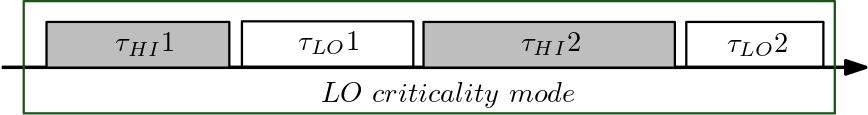
\includegraphics[width=9cm]{figs/mxsched.png}
%	\end{figure}
%	\begin{figure}
%		\centering
%		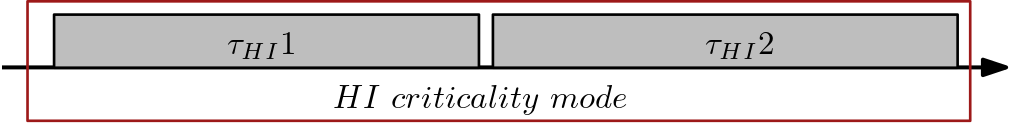
\includegraphics[width=9cm]{figs/mxschedhi.png}
%	\end{figure}
\end{frame}

\begin{frame}
	\frametitle{Limites des approches existantes}
\end{frame}

\begin{frame}
	\frametitle{Mixed-Criticality Directed Acyclic Graphs}
	\begin{columns}
		\begin{column}{0.4\textwidth}
			MC-DAG $G_j \in \mathcal{G}$.\\
			$G_j=(V_j, E_j, D_j, T_j)$.
			\begin{itemize}
				\item<2-> $V_j$ set of vertices.
				\item<3-> $E_j \subseteq (V_j \times V_j)$ set of edges.
				\item<4-> $D_j$ deadline.
				\item<5-> $T_j$ period.
			\end{itemize}
			\only<6->{Vertex $\tau_i = (\chi_i, 
			C_i(\chi_1), \dots, C_i(\chi_\ell))$}
			\begin{itemize}
				\item<6-> $\chi_i \in \mathcal{CL}$. criticality level of the 
				task.
				\item<7-> $C_i(\chi_1), \dots, C_i(\chi_\ell)$ timing 
				budgets.
			\end{itemize}
		\end{column}
		\begin{column}{0.6\textwidth}
			\begin{figure}
				\includegraphics<1|handout:0>[width=6cm]{figs/multidag_lo0.pdf}
				\includegraphics<2|handout:0>[width=6cm]{figs/multidag_lo1.pdf}
				\includegraphics<3|handout:0>[width=6cm]{figs/multidag_lo2.pdf}
				\includegraphics<4|handout:0>[width=6cm]{figs/multidag_lo3.pdf}
				\includegraphics<5|handout:0>[width=6cm]{figs/multidag_lo4.pdf}
				\includegraphics<6|handout:0>[width=6cm]{figs/multidag_lo5.pdf}
				\includegraphics<7>[width=6cm]{figs/multidag_lo.pdf}
			\end{figure}
		\end{column}
	\end{columns}
\end{frame}


%-------------------------------------------------------------------------------
\begin{frame}
	\frametitle{Integration DTIS/SEAS}
\end{frame}

%-------------------------------------------------------------------------------
\begin{frame}
	\frametitle{Bilan de candidature}
\end{frame}

\end{document} 